\begin{figure}[!ht]
    \centering
    \setlength{\resLen}{2.55in}
    \setlength{\raiseLen}{1.3in}
    \addtolength{\tabcolsep}{-4pt}
    \begin{tabular}{ccccc}
		& $\Ncls=1$ & $\Ncls=50$ & $\Ncls=100$ & $\Ncls=500$
		\\
		\raisebox{\raiseLen}{\rotatebox[origin=c]{90}{$a_i=300\text{nm}$}} &
		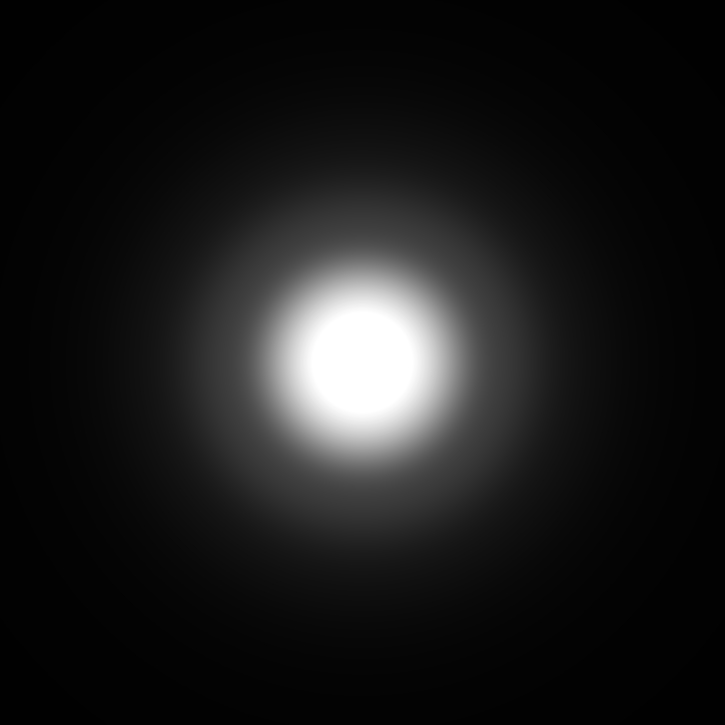
\includegraphics[height=\resLen]{waveoptics/lucy/N1_300nm.jpg} &
		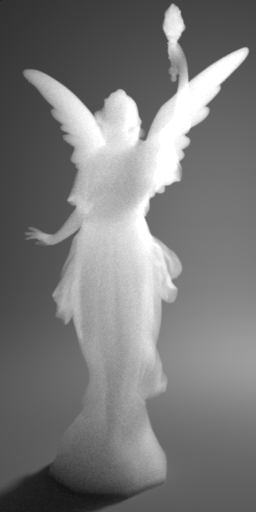
\includegraphics[height=\resLen]{waveoptics/lucy/N50_300nm.jpg} &
		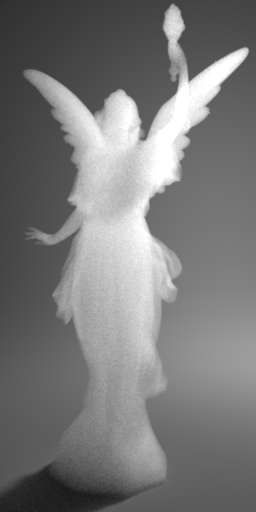
\includegraphics[height=\resLen]{waveoptics/lucy/N100_300nm.jpg} &
		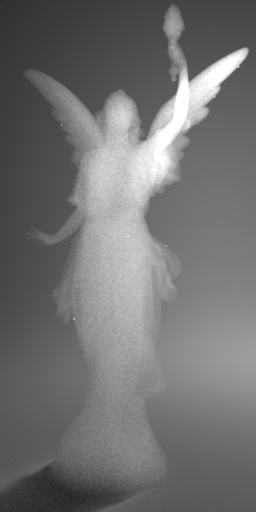
\includegraphics[height=\resLen]{waveoptics/lucy/N500_300nm.jpg}
		\\[-2pt]
		\raisebox{\raiseLen}{\rotatebox[origin=c]{90}{$a_i=400\text{nm}$}} &
		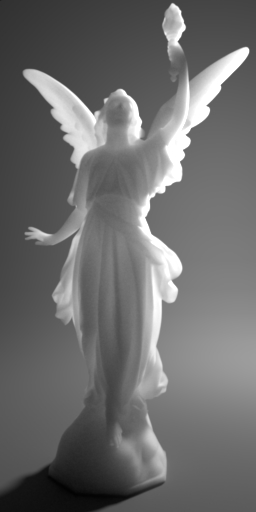
\includegraphics[height=\resLen]{waveoptics/lucy/N1_400nm.jpg} &
		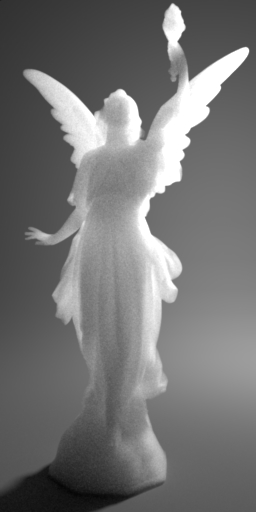
\includegraphics[height=\resLen]{waveoptics/lucy/N50_400nm.jpg} &
		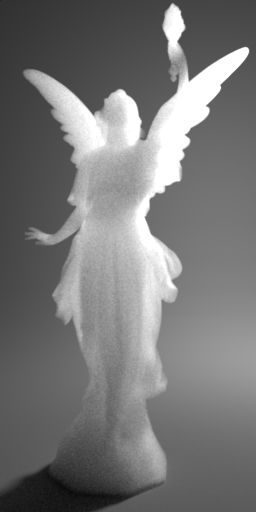
\includegraphics[height=\resLen]{waveoptics/lucy/N100_400nm.jpg} &
		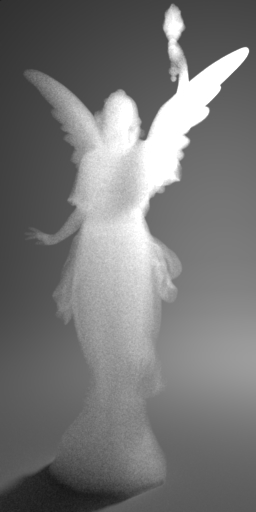
\includegraphics[height=\resLen]{waveoptics/lucy/N500_400nm.jpg}
		\\[-2pt]
		\raisebox{\raiseLen}{\rotatebox[origin=c]{90}{$a_i=500\text{nm}$}} &
		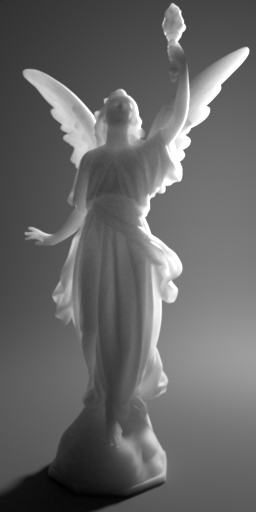
\includegraphics[height=\resLen]{waveoptics/lucy/N1_500nm.jpg} &
		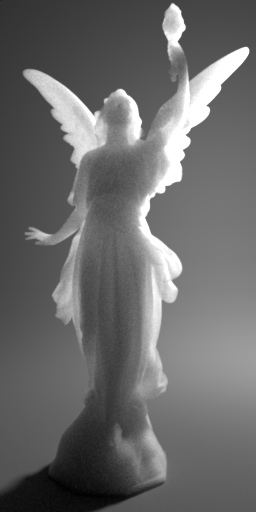
\includegraphics[height=\resLen]{waveoptics/lucy/N50_500nm.jpg} &
		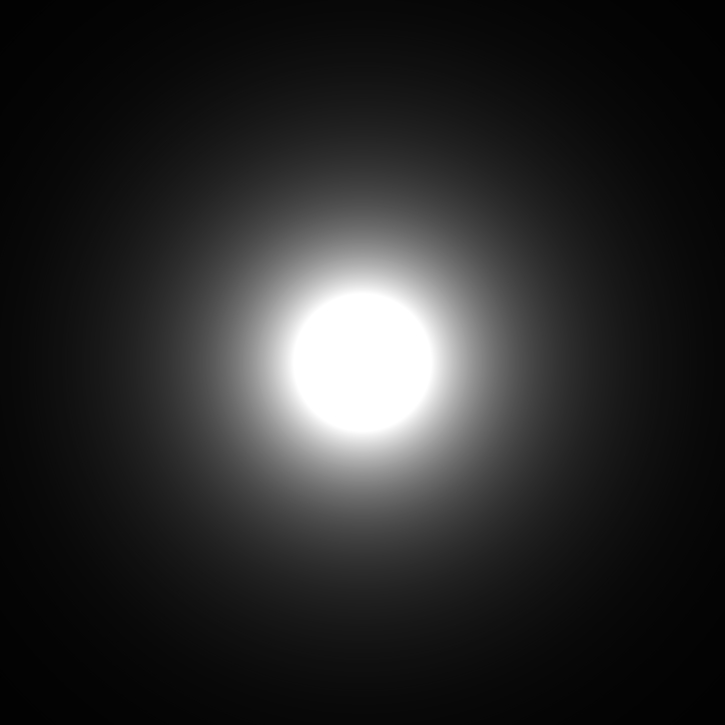
\includegraphics[height=\resLen]{waveoptics/lucy/N100_500nm.jpg} &
		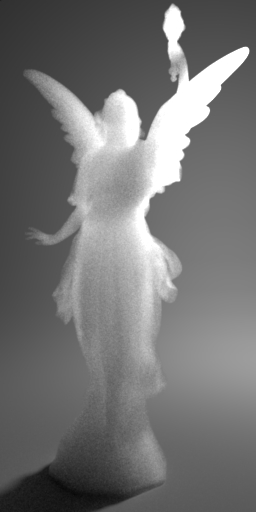
\includegraphics[height=\resLen]{waveoptics/lucy/N500_500nm.jpg} \\ [-10pt]
	\end{tabular}
    \caption[Renderings of homogeneous Lucy models]{\label{fig:waveoptics:lucycompare}
        \textbf{Renderings of homogeneous Lucy models} at $\lambda = 700\text{nm}$.
        The bulk scattering parameters are computed using our method with different combinations of particle radius $a_i$ and per-cluster particle count $\Ncls$.
    }
\end{figure}
